\documentclass{article}
	
\usepackage{thesis_style}

\bibliographystyle{ieeetr}
\graphicspath{{./img/}}
\newcommand\scalemath[2]{\scalebox{#1}{\mbox{\ensuremath{\displaystyle #2}}}}
\begin{document}
	\title{Derivation of an event-triggering rule for the fast and saturating controller}
	\author{Diogo Almeida}
	\maketitle	
	
	\section{The problem}
		We have a continuous controller proposed in \cite{lohmann_attitude}, where a Lyapunov function $V(\mathbf{x})$ is defined, as well as a resulting control signal, $\boldsymbol \tau$, defined as
		\begin{equation}
			\boldsymbol \tau = \mathbf{T(q)} - \mathbf{D(x)} \boldsymbol \omega.
			\label{tau_cont}
		\end{equation}
		
		Where the state $\mathbf{x}$ is the system attitude, $\mathbf{x} = \left [\mathbf{q} \; \boldsymbol \omega \right]$, and $V(\mathbf{x})$ is given by the sum of the kinetic energy of the system, $E_{rot}(\boldsymbol \omega)$, with an artificial potential energy $E_{pot}(\mathbf{q})$. Its time derivative is
		\[
			\dot V(\mathbf{x}) = \boldsymbol \omega^\top \boldsymbol \tau - \mathbf{T(q)}^\top \boldsymbol \omega
		\]
		and, by applying \eqref{tau_cont}, we get
		\begin{equation}
			\dot V(\mathbf{x}) = -\boldsymbol \omega^\top \mathbf{D(x)} \boldsymbol \omega,
			\label{vdot_cont}
		\end{equation}
		where $\mathbf{D(x)}$ is a positive semi-definite matrix, ensuring $\dot V(\mathbf{x}) \leq 0$.
		
		The challenge now is to find an event-triggering rule that allows for a non-periodic update of the control signal and at the same time does not permit the derivative of the Lyapunov function to grow above zero. I will use the subscript '$k$' when refering to a variable at time $t=t_k$ and no index when refering to a variable at the present time, so simplify the notation.
	\section{Definitions}
		\subsection{State error}
			Assuming that the last sampling instant is given by $t_k$, the state evolution can be given by $\mathbf{x} = \mathbf{x}_k + \mathbf{e}$, where the error $\mathbf{e}$ is defined as
			\begin{equation}
				\mathbf{e} = \mathbf{x} - \mathbf{x}_k = \begin{bmatrix}
											\mathbf{q} - \mathbf{q}_k\\
											\boldsymbol \omega - \boldsymbol \omega_k
										  \end{bmatrix} =			
										 \begin{bmatrix}
											 \mathbf{\hat{q}} \\
											  \hat{\boldsymbol \omega}
										  \end{bmatrix}
				\label{error}
			\end{equation}
		
		\subsection{Attitude quaternion}
			The proposed controler parameterizes the attitude using a quaternion, $\mathbf{q}$, that simbolizes the attitude error with respect to a given reference. Since it prioritizes the thrust direction alignment over the yaw, it further decomposes the quaternion into the product of two other quaternions, $\mathbf{q_{xy}} = \left [q_x \; q_y \; 0 \; q_p \right]^\top$  and $\mathbf{q_{z}} = \left[0\;0\;q_z\;q_w \right]^\top$. From these two quaternions we can extract the displacement angle of the thrust axis, $\varphi = 2 \arccos(q_p)$ and the yaw error angle, $\vartheta = 2 \arccos(q_w)$. 
		
		\subsection{Auxiliary function}
			Several auxiliary functions are proposed in \cite{lohmann_attitude}. In particular, $\Lambda_{\epsilon_l}^{\epsilon_u}(\epsilon)$ is of interest. It is defined as
			\begin{equation}
				\Lambda_{\epsilon_l}^{\epsilon_u}(\epsilon) = \left \{ \begin{array}{l}
												\epsilon\;\; \text{if } 0 \leq \epsilon \leq \epsilon_l\\
												\epsilon_l\;\; \text{if } \epsilon_l < \epsilon \leq \epsilon_u\\
												\epsilon_l \frac{\epsilon - \pi}{\epsilon_u - \pi}\;\; \text{if } \epsilon_u < \epsilon \leq \pi
											\end{array} \right .
				\label{lambda}
			\end{equation}
		\subsection{Artificial torque field}
			The torque field generated by the artificial potencial energy, $\mathbf{T(q)}$, is given by the sum of four fields, 
			\begin{equation}
				\mathbf{T(q)} = \mathbf{T_\varphi^\varphi(q)} + \mathbf{T_\varphi^\vartheta(q)} + \mathbf{T_\perp^\vartheta(q)} + \mathbf{T_z^\vartheta(q)}
				\label{torques}
			\end{equation}
			where
			\begin{eqnarray*}
				\mathbf{T_\varphi^\varphi(q)}  =& \displaystyle \displaystyle \frac{\displaystyle c_\varphi \Lambda_{\varphi_l}^{\varphi_u}(\varphi)}{\displaystyle\sqrt{1-q_p^2}} &\begin{bmatrix}
																		q_x\\
																		q_y\\
																		0
																	    \end{bmatrix}\\
				\mathbf{T_\varphi^\vartheta(q)}  =& \displaystyle \displaystyle \frac{\displaystyle c_\vartheta \cos^3\left (\displaystyle \frac{\varphi}{2} \right)\sin \left(\displaystyle \frac{\varphi}{2} \right) \displaystyle \int_0^\vartheta{\Lambda_{\vartheta_l}^{\vartheta_u}(\epsilon)} d\epsilon }{\displaystyle\sqrt{1-q_p^2}} &\begin{bmatrix}
										q_x\\
										q_y\\
										0
									    \end{bmatrix}\\
				\mathbf{T_\perp^\vartheta(q)}  =& \displaystyle \displaystyle \frac{\displaystyle q_z c_\vartheta \cos^3 \left(\displaystyle \frac{\varphi}{2} \right)\sin \left(\displaystyle \frac{\varphi}{2}\right) \Lambda_{\vartheta_l}^{\vartheta_u}(\vartheta)}{\displaystyle\sqrt{\displaystyle 1-q_w^2} \sqrt{\displaystyle 1-q_p^2}} &\begin{bmatrix}
										q_y\\
										-q_x\\
										0
									    \end{bmatrix}\\
				\mathbf{T_z^\vartheta(q)}  =& -\displaystyle \displaystyle \frac{\displaystyle q_z c_\vartheta \cos^4 \left(\displaystyle \frac{\varphi}{2} \right) \Lambda_{\vartheta_l}^{\vartheta_u}(\vartheta)}{\displaystyle \sqrt{\displaystyle 1-q_w^2} } &\begin{bmatrix}
											 0\\
											 0\\
											 1
										       \end{bmatrix}
			\end{eqnarray*}
		 	and, since 
		 	\begin{eqnarray*}
			 	\sin \left(\displaystyle \displaystyle \frac{\varphi}{2} \right) &=& \sqrt{1-q_p^2}\\
			 	\cos^3 \left(\displaystyle\displaystyle \frac{\varphi}{2} \right) &=& q_p^3\\
			 	\cos^4 \left(\displaystyle\displaystyle \frac{\varphi}{2} \right) &=& q_p^4
		 	\end{eqnarray*}
		 	the torque field \eqref{torques} becomes
		 	\begin{equation}
		 		\mathbf{T(q)} = \begin{bmatrix}
		 					\displaystyle \left ( \displaystyle \frac{c_\varphi \Lambda_{\varphi_l}^{\varphi_u}(\varphi)}{\sqrt{1-q_p^2}} - q_p^3 c_\vartheta \int_0^\vartheta{\Lambda_{\vartheta_l}^{\vartheta_u}(\epsilon)} d\epsilon \right ) q_x + \displaystyle \frac{q_z q_p^3 c_\vartheta \Lambda_{\vartheta_l}^{\vartheta_u}(\vartheta) q_y}{\sqrt{1-q_w^2}}\\ \\
		 					\displaystyle \left ( \displaystyle \frac{c_\varphi \Lambda_{\varphi_l}^{\varphi_u}(\varphi)}{\sqrt{1-q_p^2}} - q_p^3 c_\vartheta \int_0^\vartheta{\Lambda_{\vartheta_l}^{\vartheta_u}(\epsilon)} d\epsilon \right ) q_y - \displaystyle \frac{q_z q_p^3 c_\vartheta \Lambda_{\vartheta_l}^{\vartheta_u}(\vartheta) q_x}{\sqrt{1-q_w^2}}\\ \\
							\displaystyle \displaystyle \frac{q_z q_p^4 c_\vartheta \Lambda_{\vartheta_l}^{\vartheta_u}(\vartheta)}{\sqrt{1-q_w^2}}	 		
		 				\end{bmatrix}
		 		\label{torques_vec}
		 	\end{equation}

	\section{Rule derivation}
		Using an event-triggering rule, $\boldsymbol \tau = \boldsymbol \tau_k$, equation \eqref{vdot_cont} does not hold anymore. Instead, we have
		\[
			\dot V(\mathbf{x}) = \boldsymbol \omega^\top \boldsymbol \tau_k - \mathbf{T(q})^\top\boldsymbol \omega
		\]
		and, by recalling $\mathbf{x} = \mathbf{x}_k + \mathbf{e}$, together with \eqref{error} and \eqref{tau_cont}
		\[
			\dot V(\mathbf{x}_k+\mathbf{e}) = \boldsymbol \omega^\top \left [ \mathbf{T(q}_k) - \mathbf{T(q}_k + \mathbf{\hat{q}}) \right ] - \boldsymbol \omega_k^\top \mathbf{D(x}_k) \boldsymbol \omega_k -  \hat{\boldsymbol \omega}^\top \mathbf{D(x}_k) \boldsymbol \omega_k.
		\]
		
		The term $-\boldsymbol \omega_k^\top \mathbf{D(x}_k) \boldsymbol \omega_k = \dot V(\mathbf{x}_k)$ is always $\leq 0$, as it is constant and obtained as in \cite{lohmann_attitude}. $\hat{\boldsymbol \omega}^\top \mathbf{D(x}_k) \boldsymbol \omega_k$ has $\hat{\boldsymbol \omega}$ as the only variable, making it easy to monitor. The subtraction $\mathbf{T(q}_k) - \mathbf{T(q}_k + \mathbf{\hat{q}})$ is the operation that is harder to compute, since it involves constantly doing the computations \eqref{torques_vec}. It is possible to linearize $\mathbf{T(q)}$ around $\mathbf{q}_k$ to obtain an expression that is linear in an error term:
		\begin{equation}
			\mathbf{T(q}_k+\mathbf{\hat{q}}) \simeq \mathbf{T(q}_k) +  \nabla \mathbf{T(\hat{q}}) 
			\label{lin_torque} 
		\end{equation}
		where
		\[
			\displaystyle \nabla \mathbf{T(\hat{q}}) =\left .\displaystyle \frac{\partial T}{\partial q_x}\right |_{t=t_k}\hat{q}_x +
								\left .\displaystyle \frac{\partial T}{\partial q_y}\right |_{t=t_k}\hat{q}_y +
								\left .\displaystyle \frac{\partial T}{\partial q_z}\right |_{t=t_k}\hat{q}_z +
								\left .\displaystyle \frac{\partial T}{\partial q_p}\right |_{t=t_k}\hat{q}_p +
								\left .\displaystyle \frac{\partial T}{\partial q_w}\right |_{t=t_k}\hat{q}_w				
		\]
		Using \eqref{lin_torque}, $\dot V(\mathbf{x}_k + \mathbf{e})$ becomes
		\[
			\dot V(\mathbf{x}_k + \mathbf{e}) = -\boldsymbol \omega^\top  \nabla \mathbf{T(\hat{q}}) + \dot V(\mathbf{x}_k) - \hat{\boldsymbol \omega}(t)^\top \mathbf{D(x}_k) \boldsymbol \omega_k
		\]
		and, by ensuring
		\begin{equation}
			\boldsymbol \omega^\top  \nabla \mathbf{T(\hat{q}}) + \hat{\boldsymbol \omega}(t)^\top \mathbf{D(x}_k) \boldsymbol \omega_k \leq \dot V(\mathbf{x}_k) 
			\label{trigger}
		\end{equation}
		we get $\dot V(\mathbf{x}(t)) \leq 0$.
		
	\section{Simulation}
		\begin{figure}[H]
			\centering
			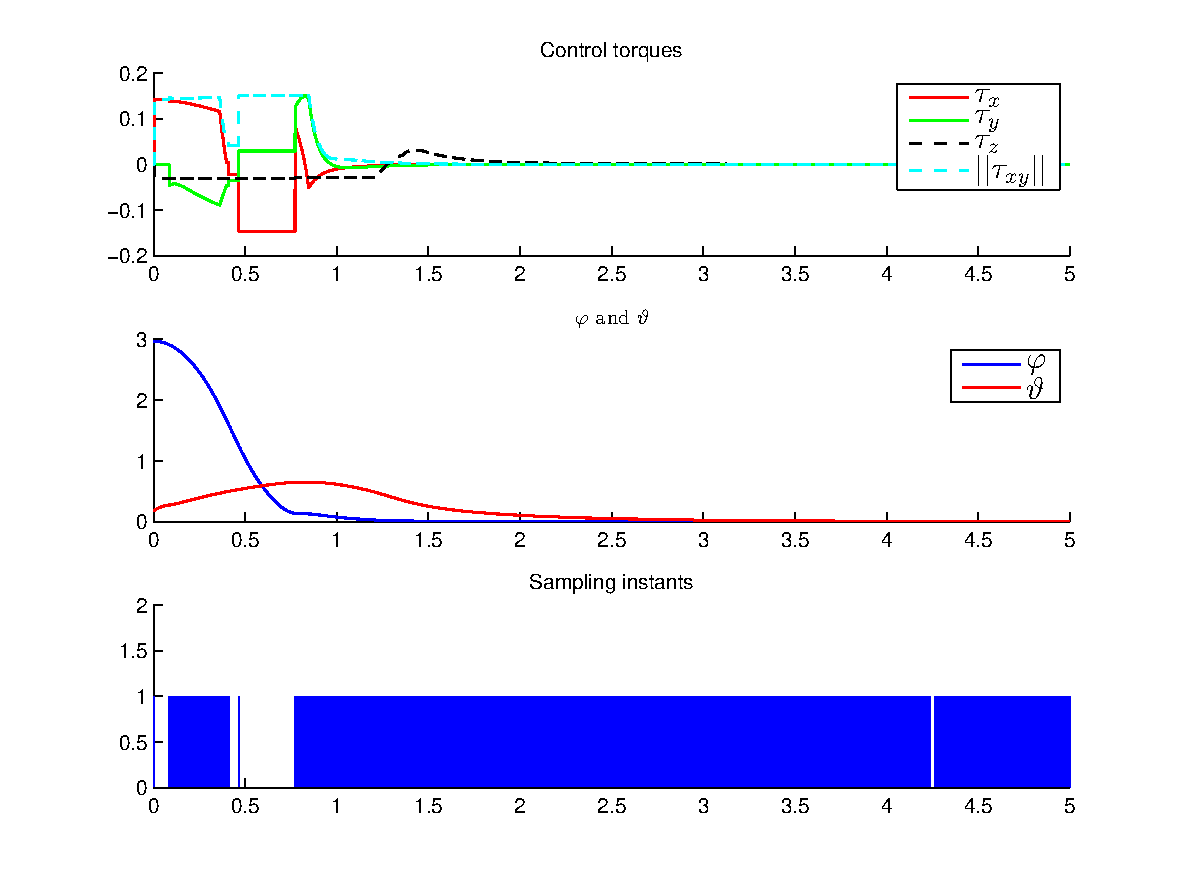
\includegraphics[width=\textwidth]{event1}
			\caption{Resulting control torques and system behavior using rule \eqref{trigger}\label{event_fig}}
		\end{figure}
		
		\begin{figure}[H]
			\centering
			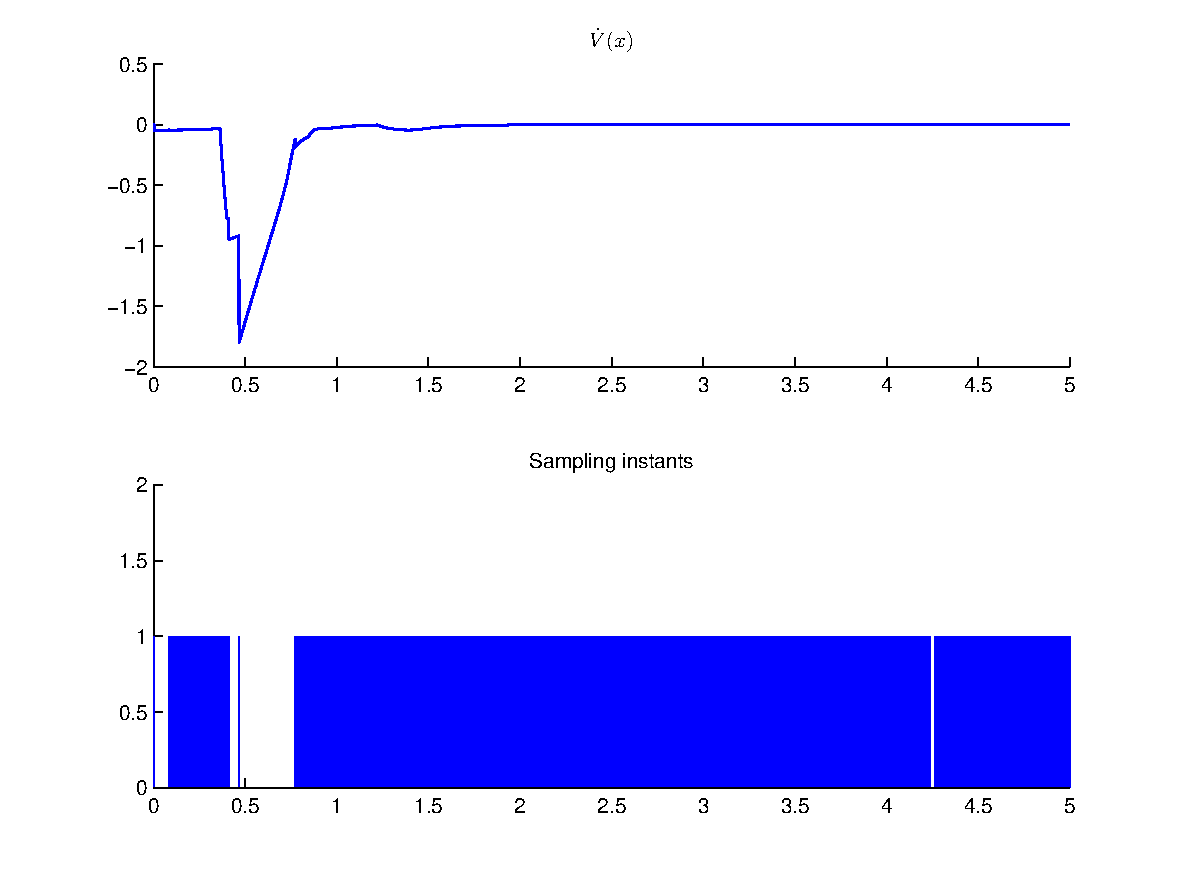
\includegraphics[width=\textwidth]{lyapu}
			\caption{$\dot V(\mathbf{x})$ evolution\label{lyapu_fig}}
		\end{figure}
		
\bibliography{thesis_bib}
%===================================================================================================================================
\appendix
	\section{$\nabla \mathbf{T(\hat{q}})$ derivation}
		We need to compute the partial derivatives that composes $\nabla \mathbf{T(\hat{q}})$ in order to apply \eqref{trigger}. With:
		\begin{eqnarray*}
			A &=& \sqrt{1-q_{w_k}^2}\\\\
			B &=& c_\vartheta \displaystyle \int_0^{\vartheta_k}{\Lambda_{\vartheta_l}^{\vartheta_u}(\epsilon)} d\epsilon\\\\
			C &=& \displaystyle \displaystyle \frac{c_\varphi}{\sqrt{1-q_{p_k}^2}}\\\\
			D &=& \displaystyle \displaystyle \frac{c_\vartheta}{A}\\\\
			E &=& \arccos(q_{w_k}) \\\\
			F &=& \arccos(q_{p_k})
		\end{eqnarray*}
		we have:
		
		\begin{eqnarray*}
				\left .\displaystyle \frac{\partial T}{\partial q_x}\right |_{t=t_k}  =& \begin{bmatrix}
												C \Lambda_{\varphi_l}^{\varphi_u}(\varphi_k) - q_{p_k}^3 B \\\\
												-q_{z_k} q_{p_k}^3 D \Lambda_{\vartheta_l}^{\vartheta_u}(\vartheta_k)\\\\
												0
											   \end{bmatrix}
											   \\
				\left .\displaystyle \frac{\partial T}{\partial q_y}\right |_{t=t_k}  =& \begin{bmatrix}
												q_{z_k} q_{p_k}^3 D \Lambda_{\vartheta_l}^{\vartheta_u}(\vartheta_k) \\\\
												C \Lambda_{\varphi_l}^{\varphi_u}(\varphi_k) - q_{p_k}^3 B\\\\
												0
											   \end{bmatrix}
											   \\
				\left .\displaystyle \frac{\partial T}{\partial q_z}\right |_{t=t_k}  =& \begin{bmatrix}
												q_{y_k} q_{p_k}^3 D \Lambda_{\vartheta_l}^{\vartheta_u}(\vartheta_k)\\\\
												q_{x_k} q_{p_k}^3 D \Lambda_{\vartheta_l}^{\vartheta_u}(\vartheta_k)\\\\
												q_{p_k}^4 D \Lambda_{\vartheta_l}^{\vartheta_u}(\vartheta_k)
											   \end{bmatrix}.
		\end{eqnarray*}
		
		$\left .\displaystyle \frac{\partial T}{\partial q_p}\right |_{t=t_k}$ and $\left .\displaystyle \frac{\partial T}{\partial q_w}\right |_{t=t_k}$ will depend on the value of $\varphi$ and $\vartheta$, respectively, due to \eqref{lambda}. Since $\displaystyle \frac{\partial \varphi}{\partial q_p} = - \displaystyle \frac{2}{\sqrt{1-q_p^2}}$, we have, for $0 \leq \varphi < \varphi_l$:
		\[
			\left .\displaystyle \frac{\partial T}{\partial q_p}\right |_{t=t_k}  = \begin{bmatrix}
												\left (\displaystyle \frac{-4 C F}{A} + \displaystyle \frac{q_{p_k} C}{A^2}- 3 q_{p_k}^2 B \right )q_{x_k} + 3 q_{z_k} q_{y_k} q_{p_k}^2 D \Lambda_{\vartheta_l}^{\vartheta_u}(\vartheta_k)\\\\
												\left (\displaystyle \frac{-4 C F}{A} + \displaystyle \frac{q_{p_k} C}{A^2} - 3 q_{p_k}^2 B \right )q_{y_k} - 3 q_{z_k} q_{x_k} q_{p_k}^2 D \Lambda_{\vartheta_l}^{\vartheta_u}(\vartheta_k)\\\\
												4 q_{z_k} q_{p_k}^3 D \Lambda_{\vartheta_l}^{\vartheta_u}(\vartheta_k)
											   \end{bmatrix}
		\] 
		for $\varphi_l \leq \varphi < \varphi_u$:
		\[
			\left .\displaystyle \frac{\partial T}{\partial q_p}\right |_{t=t_k}  = \begin{bmatrix}
												\left ( \varphi_lC -3 q_{p_k}^2 B \right )q_{x_k} + 3 q_{z_k} q_{y_k} q_{p_k}^2 D \Lambda_{\vartheta_l}^{\vartheta_u}(\vartheta_k)\\\\
												\left ( \varphi_lC -3 q_{p_k}^2 B \right )q_{y_k} -3 q_{z_k} q_{x_k} q_{p_k}^2 D \Lambda_{\vartheta_l}^{\vartheta_u}(\vartheta_k)\\\\
												4 q_{z_k} q_{p_k}^3 D \Lambda_{\vartheta_l}^{\vartheta_u}(\vartheta_k)
											   \end{bmatrix}
		\] 
		and, for $\varphi_u \leq \varphi < \pi$:
		\[
			\left .\displaystyle \frac{\partial T}{\partial q_p}\right |_{t=t_k}  = \begin{bmatrix}
												\left (\displaystyle \frac{C \varphi_l q_{p_k} \left ( 2F -\pi \right)}{A^2 \left ( \varphi_u - \pi \right )}-\displaystyle \frac{2 C \varphi_l}{\left (\varphi_u-\pi \right)A} - 3 q_{p_k}^2 B \right )q_{x_k} + 3 q_{z_k} q_{y_k} q_{p_k}^2 D \Lambda_{\vartheta_l}^{\vartheta_u}(\vartheta_k)\\\\
												\left (\displaystyle \frac{C \varphi_l q_{p_k} \left ( 2F -\pi \right)}{A^2 \left ( \varphi_u - \pi \right )}-\displaystyle \frac{2 C \varphi_l}{\left (\varphi_u-\pi \right) A} - 3 q_{p_k}^2 B \right )q_{y_k} - 3 q_{z_k} q_{x_k} q_{p_k}^2 D \Lambda_{\vartheta_l}^{\vartheta_u}(\vartheta_k)\\\\
												4 q_{z_k} q_{p_k}^3 D \Lambda_{\vartheta_l}^{\vartheta_u}(\vartheta_k)
											   \end{bmatrix}
		\] 
		
		For $\vartheta = 2\arccos(q_w)$ we get $\displaystyle \frac{\partial \vartheta}{\partial q_w} = -\displaystyle \frac{2}{\sqrt{1-q_w^2}}$ and $\displaystyle \frac{\partial (\vartheta)^2}{\partial q_w} = -\displaystyle \frac{8\arccos(q_w)}{\sqrt{1-q_w^2}}$. When $0 \leq \vartheta < \vartheta_l$, $\int_0^{\vartheta(t)}{\Lambda_{\vartheta_l}^{\vartheta_u}(\epsilon)} d\epsilon = \displaystyle \frac{\vartheta^2}{2}$ and, as such:
		\[
			\left .\displaystyle \frac{\partial T}{\partial q_w}\right |_{t=t_k}  = \begin{bmatrix}
											4 q_{p_k}^3 q_{x_k} D  + \displaystyle \frac{2 q_{w_k} q_{z_k} q_{p_k}^3 q_{y_k} D E}{A^2} - \displaystyle \frac{2 q_{z_k} q_{p_k}^3 q_{y_k} C}{A}\\
											4 q_{p_k}^3 q_{y_k} D - \displaystyle \frac{2 q_{w_k} q_{z_k} q_{p_k}^3 q_{x_k} D E}{A^2} + \displaystyle \frac{2 q_{z_k} q_{p_k}^3 q_{x_k} C}{A}\\
											\displaystyle \frac{2 q_{z_k} q_{p_k}^4 q_{w_k} D E}{A^2} - \displaystyle \frac{2 q_{z_k} q_{p_k}^4 D}{A}
										\end{bmatrix} 
		\]
		
		When $\vartheta_l \leq \vartheta < \vartheta_u$, $\int_0^{\vartheta(t)}{\Lambda_{\vartheta_l}^{\vartheta_u}(\epsilon)} d\epsilon = \displaystyle \frac{\vartheta_l^2}{2} + \vartheta_l \left ( \vartheta-\vartheta_l \right )$:
		
		\[
			\left .\displaystyle \frac{\partial T}{\partial q_w}\right |_{t=t_k}  = \begin{bmatrix}
											2 \vartheta_l q_{p_k}^3 q_{x_k} D + \displaystyle \frac{\vartheta_l q_{w_k} q_{z_k} q_{p_k}^3 q_{y_k} \left (2 E-\vartheta_l \right ) D}{A^2} - \displaystyle \frac{2 \vartheta_l  q_{z_k} q_{p_k}^3 q_{y_k} D}{A}\\
											2 \vartheta_l q_{p_k}^3 q_{y_k} D - \displaystyle \frac{\vartheta_l q_{w_k} q_{z_k} q_{p_k}^3 q_{x_k}  \left (2 E-\vartheta_l \right )  D}{A^2} + \displaystyle \frac{2 \vartheta_l q_{z_k} q_{p_k}^3 q_{x_k} D}{A}\\
											\displaystyle \frac{\vartheta_l q_{z_k} q_{p_k}^4 q_{w_k} \left (2 E-\vartheta_l \right ) D}{A^2} - \displaystyle \frac{2 \vartheta_l q_{z_k} q_{p_k}^4 D}{A}
										\end{bmatrix} 
		\]
		
		Finally, for $\vartheta_u \leq \vartheta \leq \pi$, the integral becomes $\displaystyle \frac{\vartheta_l^2}{2} + \vartheta_l \left(\vartheta_u-\vartheta_l \right) + \displaystyle \frac{\vartheta_l \left (\vartheta^2 - \vartheta_u^2 \right)}{2\left(\vartheta_u - \pi \right )} + \displaystyle \frac{\vartheta_l \pi \left ( \vartheta_u - \vartheta \right)}{\vartheta_u - \pi}$ and the last partial derivative is
		
		\[
			\left .\displaystyle \frac{\partial T}{\partial q_w}\right |_{t=t_k}  = 
										\begin{bmatrix}
											-\displaystyle \frac{\vartheta_l q_{p_k}^3 q_{x_k} \left (2\pi-4 E \right) D}{\vartheta_u - \pi } + \displaystyle \frac{\vartheta_l q_{w_k} q_{z_k} q_{p_k}^3 q_{y_k} \left (2 E-\pi \right ) D}{\left (\vartheta_u - \pi \right )A^2} - \displaystyle \frac{2 \vartheta_l q_{z_k} q_{p_k}^3 q_{y_k} D}{\left(\vartheta_u - \pi \right )A}\\
											-\displaystyle \frac{\vartheta_l q_{p_k}^3 q_{y_k} \left (2\pi-4 E \right) D}{\vartheta_u - \pi} - \displaystyle \frac{\vartheta_l q_{w_k} q_{z_k} q_{p_k}^3 q_{x_k} \left (2 E-\pi \right ) D}{\left (\vartheta_u - \pi \right )A^2} + \displaystyle \frac{2 \vartheta_l q_{z_k} q_{p_k}^3 q_{x_k} D}{\left(\vartheta_u - \pi \right )A}\\
											\displaystyle \frac{\vartheta_l q_{z_k} q_{p_k}^4 q_{w_k} \left (2 E-\pi \right ) D}{\left(\vartheta_u-\pi \right)A^2} - \displaystyle \frac{2 \vartheta_l q_{z_k} q_{p_k}^4 D}{\left ( \vartheta_u - \pi \right )A}
										\end{bmatrix} 
		\]
\end{document}
